\chapter{LTE}

\section{Deux équations}

L'équation du transport de la lumière \textit{LTE} (Light Transport Equation) décrit la distribution de la radiance dans toute la scène. Elle permet de connaître la radiance réfléchie en un point d'une surface, en fonction de l'émission de cette surface, sa BRDF et toutes les autres surfaces de la scène pouvant venir perturber le rayon.\newline\par

Il existe deux LTE différentes : l'équation de \textit{rendu} et l'équation en \textit{potentiel}. Dans l'équation de rendu, les rayons étudiés partent du récepteur et on cherche des chemins remontant jusqu'aux sources. L'équation de potentiel partage le même principe mais dans l'autre sens, les rayons étant tiré de la source et on calcule leur contributions sur le récepteur.\par
Dans les deux cas, il s'agit de trouver l'éclairage global de la scène et non pas juste l'éclairage direct qui ne prend en compte que les rayons provenant directement d'une source de lumière. Ici, on souhaite également tenir compte de la radiance provenant de réflexions sur des surfaces n'étant pas forcément auto-émittante.\newline\par

L'\textbf{équation de rendu} s'exprime par la formule :
\large \begin{equation}\label{eq:LTE_rendu}
    L_r(x, \overrightarrow{\omega_r}, t) =
        L_e(x, \overrightarrow{\omega_r}, t) +
        \int_{\Omega_x}
            f_r(x, \overrightarrow{\omega_i} \longrightarrow \overrightarrow{\omega_r})
            L_i(x, \overrightarrow{\omega_i}, t)
            |\overrightarrow{\omega_i}, \overrightarrow{n} |
        d\overrightarrow{\omega_i}
,\end{equation} \normalsize
où $L_e(x, \overrightarrow{\omega_r}, t)$ est la lumière auto-émise par la surface, \\
$L_i(x, \overrightarrow{\omega_i}, t)$ est la radiance incidente dans la direction $\overrightarrow{\omega_i}$, \\
$\overrightarrow{n}$ est la normale à la surface au point $x$, \\
$f_r(x, \overrightarrow{\omega_i} \longrightarrow \overrightarrow{\omega_r})$ est la BRDF de la surface au point x dans le sens de propagation $\overrightarrow{\omega_i} \longrightarrow \overrightarrow{\omega_r}$.\newline\par

L'\textbf{équation en potentiel} s'exprime par la formule :
\large \begin{equation} \label{eq:LTE_potentiel}
    W(x, y, \overrightarrow{\omega_x}, t) =
        W_e(x, y, \overrightarrow{\omega_x}, t) +
        \int_{\Omega_z}
            f_r(z, \overrightarrow{\omega_x} \longrightarrow \overrightarrow{\omega_z})
            W(z, y, \overrightarrow{\omega_z}, t)
            |\overrightarrow{\omega_z}, \overrightarrow{n_z} |
        d\overrightarrow{\omega_z}
,\end{equation} \normalsize
où $W(x, y, \overrightarrow{\omega_x}, t)$ est l'action potentielle du point $x$ sur le point $y$ dans la direction $\overrightarrow{\omega_x}$, \\
$ W_e(x, y, \overrightarrow{\omega_x}, t)$ est l'action potentielle directe de la source au point $x$ sur le point $y$ suivant $\overrightarrow{\omega_x}$.\par
Dans ce rapport et pour ce qui suit, je me place dans le cas de l'équation en potentiel.

\section{Equation en potentiel avec réflexions}

L'éclairement reçu au niveau d'un récepteur positionné en $M_{rx}$ pour un rayonnement émis par une source positionnée en $M_{tx}$ est donné par :
\large \begin{equation}
    E(M_{tx}, M_{rx}, t) =
        \int_{\Omega_{tx}}
            L_e(M_{tx}, \overrightarrow{\omega_0}, t)
            W(M_{tx}, M_{rx}, \overrightarrow{\omega_0}, t)
            | \overrightarrow{\omega_0} \cdot \overrightarrow{n_{tx}} |
        d\overrightarrow{\omega_0}
,\end{equation} \normalsize
où $L_e(M_{tx}, \overrightarrow{\omega_0}, t)$ désigne le rayonnement sortant dans la direction $\overrightarrow{\omega_0}$.\newline\par

Cela dit, la plupart des rayons lancés de la source ne vont pas directement au récepteur et sont d'abord réfléchis par des surfaces. Aussi, après $k$ réflexions, nous avons l'équation suivante :
\large \begin{equation}
    E_k(M_{tx}, M_{rx}, t) =
        \int_{\Omega_{tx}} \cdots
            \int_{\Omega_k}
                f_k(\bar{x}, t)
            d\overrightarrow{\omega_0}
            \cdots
        d\overrightarrow{\omega_k}
,\end{equation} \normalsize
où $\bar{x}$ correspond au trajet de propagation de la lumière entre $M_{tx}$ et $M_{rx}$ rebondissant sur les $x_i$ points de réflexions ($i \in \llbracket1, k\rrbracket$). Et 
\large \begin{multline}
    f_k(\bar{x}, t) =
        | \overrightarrow{\omega_0} \cdot \overrightarrow{n_{tx}} |
        L_e(M_{tx}, \overrightarrow{\omega_0}, t)
        rect\left(
            \frac
                {| \overrightarrow{x_k M{rx}} \cdot \overrightarrow{n_{rx}} |}
                {cos(FOV) \Vert \overrightarrow{x_k M_{rx}}}
        \right)
        W_l(x_k, M_{rx}, \overrightarrow{\omega_k} t) \\
        \times
        \prod\limits_{i=1}^k
            f_r(x_i, \overrightarrow{\omega_{i-1}} \longrightarrow \overrightarrow{\omega_i})
            | \overrightarrow{\omega_i} \cdot \overrightarrow{n_i} |
,\end{multline} \normalsize
avec la fonction $rect$ qui vérifie que $x_k$ est dans le champ de vision du récepteur et $W_l(x_k, M_{rx}, t)$ qui est l'action potentielle directe du dernier point de réflexion $x_k$ sur le récepteur.

\section{Equation en potentiel optimisée}
\label{sec:LTE}

L'équation précédente permet seulement de suivre un chemin de $k$ réflexions puis de regarder l'action potentielle sur le récepteur du dernier point $x_k$ du chemin. De ce fait, les actions potentielles des points de réflexions $x_i$ ($1 \leq i < k$) doivent être calculés indépendemment les uns des autres, et nous aurons à lancer $k$ fois le même chemin (de plus en plus long) pour avoir les $k$ contributions.\newline\par

Une optimisation possible de l'équation cherche donc à ne pas répéter inutilement les réflexions. Elle consiste à calculer, pour chaque point $x_i$ son action potentielle sur le récepteur dès le premier lancé de rayon. Cette technique s'appelle l'\textit{estimation du prochain évènement} (NEE "Next Event Estimation"). Ces contributions sont représentées dans la figure \ref{fig:LTE_potentiel} par les traits en pointillés reliant un point de réflexion $x_i$ à un récepteur $M_{rx}$.\newline

\begin{figure}[h!]\label{fig:LTE_potentiel}
\centering
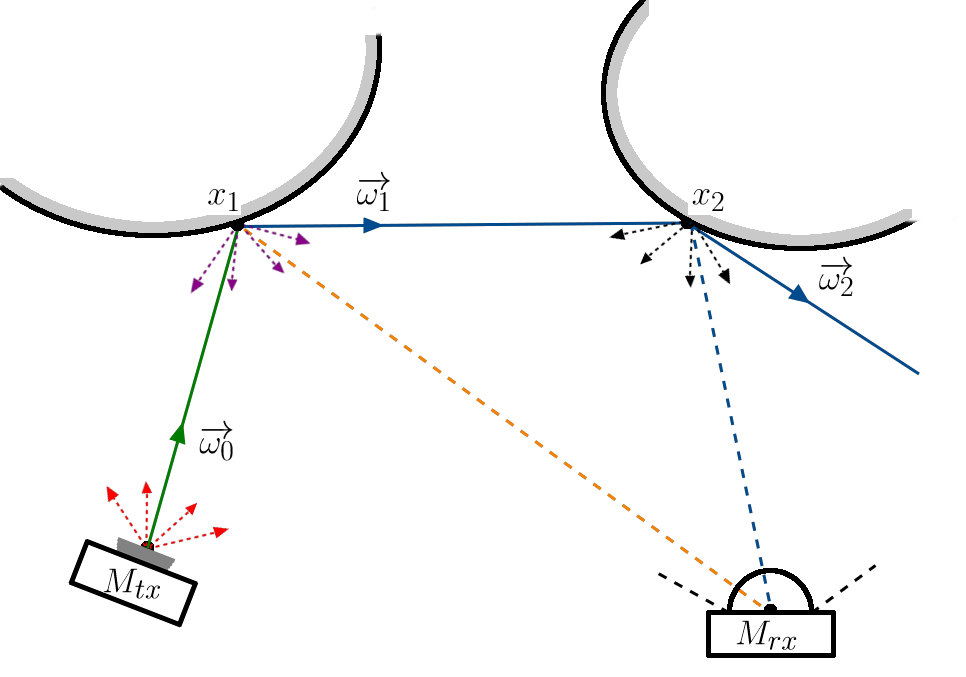
\includegraphics[width=150mm]{LTE.png}
\caption{Équation en potentiel avec la technique NEE}
\end{figure}


\large
\begin{equation}
    E(M_{tx}, M_{rx}, t) = \int_{\Omega_{tx}}
        \underbrace{\textcolor{OliveGreen}{L_e(M_{tx}, \overrightarrow{\omega_0}, t)}}
            _{\textcolor{DarkGray}
             {\substack{\text{rayonnement sortant} \\
                        \text{de $M_{tx}$ dans} \\
                        \text{la direction $\overrightarrow{\omega_0}$}}}}
        \underbrace{W(M_{tx}, M_{rx}, \overrightarrow{\omega_0}, t)}
            _{\textcolor{DarkGray}
             {\substack{\text{action potentielle de} \\
                        \text{la source $M_{tx}$ sur} \\
                        \text{le récepteur $M_{rx}$} \\
                        \text{dans la direction $\overrightarrow{\omega_0}$}}}}
        | \overrightarrow{\omega_0} \cdot \overrightarrow{n_{tx}} |
        \underbrace{\textcolor{red}{d\overrightarrow{\omega_0}}}
            _{\textcolor{DarkGray}
             {\substack{\text{intégrale} \\
                        \text{sur le} \\
                        \text{domaine} \\
                        \text{des} \\
                        \text{directions}}}}
.\end{equation} \normalsize

On tire un rayon de la source $M_{tx}$ dans la direction $\overrightarrow{\omega_0}$. Bien évidemment nous avons le rayonnement $L_e(M_{tx}, \overrightarrow{\omega_0}, t)$ sortant de la source, rayonnement atténué selon son inclinaison par rapport à la normale $\overrightarrow{n_{tx}}$ de la source. Ce rayonnement n'atteignant pas forcément le récepteur $M_{rx}$ immédiatement, il faut donc calculer l'action potentielle $W(M_{tx}, M_{rx}, \overrightarrow{\omega_0}, t)$ que la source a sur le récepteur par la direction $\overrightarrow{\omega_0}$.

\large \begin{multline}
    E(M_{tx}, M_{rx}, t) = \int_{\Omega_{tx}}
        \textcolor{OliveGreen}{L_e(M_{tx}, \overrightarrow{\omega_0}, t)}
        | \overrightarrow{\omega_0} \cdot \overrightarrow{n_{tx}} | \\
        \times \left(
        \underbrace{\textcolor{BurntOrange}{W_l^*(x_1, M_{rx}, t)}}
            _{\textcolor{DarkGray}
             {\substack{\text{contribution directe} \\
                        \text{de $x_1$ sur $M_{rx}$, en} \\
                        \text{tenant compte de la} \\
                        \text{BDRF}}}}
        + \int_{\Omega_1}
        \underbrace{\textcolor{blue}{W^*(x_1, M_{rx}, \overrightarrow{\omega_1}, t)}}
            _{\textcolor{DarkGray}
             {\substack{\text{contribution dans la direction} \\
                        \text{$\overrightarrow{\omega_1}$ en repartant de $x_1$} \\
                        \text{(à dérouler)}}}}
        \textcolor{purple}{d\overrightarrow{\omega_1}}
        \right)
        \textcolor{red}{d\overrightarrow{\omega_0}}
,\end{multline} \normalsize
avec
\large \begin{equation}
    W^*(x_1, M_{rx}, \overrightarrow{\omega_1}, t) = 
        f_r(x_1, \overrightarrow{\omega_0} \longrightarrow \overrightarrow{\omega_1})
        W(x_1, M_{rx}, \overrightarrow{\omega_1}, t)
        | \overrightarrow{\omega_1} \cdot \overrightarrow{n_1} |
,\end{equation} \normalsize
et
\large \begin{equation}
    W_l^*(x_1, M_{rx}, t) =
        f_r(x_1, \overrightarrow{\omega_0} \longrightarrow \overrightarrow{x_1 M_{rx}})
        W_l(x_1, M_{rx}, t)
        | \overrightarrow{\omega_1} \cdot \overrightarrow{n_1} |
.\end{equation} \normalsize

L'action potentielle $W(M_{tx}, M_{rx}, \overrightarrow{\omega_0}, t)$ se calcule en deux termes. Premièrement, sachant qu'en partant dans la direction $\overrightarrow{\omega_0}$ à partir du point $M_{tx}$ le rayon intercepte une surface au point de réflexion $x_1$, il faut regarder la contribution directe sur le récepteur de la lumière réfléchie en ce point; il s'agit du terme $W_l^*(x_1, M_{rx}, t)$. Ce premier terme ne traite donc que la direction de réflexion $\overrightarrow{x_1 M_{rx}}$.\par
Hors il y a tout un hémisphère de directions $\overrightarrow{\omega_1}$ possibles qu'il faut regarder. C'est ce que se charge de faire le deuxième terme $\int_{\Omega_1}W^*(x_1, M_{rx}, \overrightarrow{\omega_1}, t)d\overrightarrow{\omega_1}$. Ce terme là continue donc les chemins possibles du rayon et parmi toutes les directions, certaines iront intercepter d'autres surfaces (la direction $\omega_1$ qui intercepte une surface au point $x_2$ par exemple, sur la figure \ref{fig:LTE_potentiel}). C'est donc sur celui-ci qu'il faudra dérouler l'équation pour avoir $E_k(M_{tx}, M_{rx}, t)$.

\large \begin{multline} \label{eq:Eclairement_LTE_potentiel}
    E(M_{tx}, M_{rx}, t) =
        \int_{\Omega_{tx}}
            \textcolor{OliveGreen}{L_e(M_{tx}, \overrightarrow{\omega_0}, t)}
            \textcolor{BurntOrange}{W_l^*(x_1, M_{rx}, t)}
            | \overrightarrow{\omega_0} \cdot \overrightarrow{n_{tx}} |
            \textcolor{red}{d\overrightarrow{\omega_0}}
        \\ +
        \int_{\Omega_{tx}}
            \textcolor{OliveGreen}{L_e(M_{tx}, \overrightarrow{\omega_0}, t)}
            | \overrightarrow{\omega_0} \cdot \overrightarrow{n_{tx}} |
            \int_{\Omega_1}
                \textcolor{blue}{W^*(x_1, M_{rx}, \overrightarrow{\omega_1}, t)}
            \textcolor{red}{d\overrightarrow{\omega_0}}
        \textcolor{purple}{d\overrightarrow{\omega_1}}
.\end{multline} \normalsize

En séparant l'intégrale sur $\Omega_{tx}$ en deux intégrales, avec une seule à dérouler, nous pouvons facilement écrire l'équation pour $k$ réflexions.

\large \begin{equation}
\begin{split}
    E_k(M_{tx}, M_{rx}, t) =
        &\int_{\Omega_{tx}}
            f_1({M_{tx}, x_1, M_{rx}}, t)
        d\overrightarrow{\omega_0}
        \\ &+
        \int_{\Omega_{tx}}
            \int_{\Omega_1}
                f_2({M_{tx}, x_1, x_2,  M_{rx}}, t)
            d\overrightarrow{\omega_0}
        d\overrightarrow{\omega_1}
        \\ &\vdots
        \\ &+
        \int_{\Omega_{tx}}
            \cdots
            \int_{\Omega_k}
                f_k(\bar{x}, t)
            d\overrightarrow{\omega_0}
            \cdots
        d\overrightarrow{\omega_k}
.\end{split}
\end{equation} \normalsize \newline\par

Avec les intégrales sur les domaines de chemin, il est facile de voir que cette équation est très facilement transformable avec la méthode de Monte Carlo pour des facilités algorithmiques :
\large \begin{multline}
    E_k(M_{tx}, M_{rx}, t) =
    \frac{1}{N}
    \underbrace{
        \sum\limits_{s=1}^N \frac
            {| \overrightarrow{\omega_0} \cdot \overrightarrow{n_{tx}} |
             L_e(M_{tx}, \overrightarrow{\omega_{tx}}, t)}
            {p_0(M_{tx}, \overrightarrow{\omega_0})}
        }
        _{\textcolor{DarkGray}
         {\substack{\text{On tire une première} \\
                    \text{direction pour $\overrightarrow{\omega_0}$}}}}
    \\ \times
    \sum \limits_{i=1}^k
    \left(
        \underbrace
            {W_l(x_i, M_{rx}, t)}
            _{\textcolor{DarkGray}
             {\substack{\text{Contribution} \\
                        \text{directe du} \\
                        \text{point $x_i$ sur} \\
                        \text{le récepteur}}}}
        \underbrace
            {\prod\limits_{j=1}^i
                \frac
                    {f_r(x_j, \overrightarrow{\omega_{j-1}} \longrightarrow \overrightarrow{\omega_{j}})
                    | \overrightarrow{\omega_j} \cdot \overrightarrow{n_j} |}
                    {p_j(x_j, \overrightarrow{\omega_{j}})}}
                _{\textcolor{DarkGray}
                 {\substack{\text{Prise en compte de toutes} \\
                            \text{les BRDF des surfaces interceptées} \\
                            \text{par le chemin aux points $x_i$}}}}
    \right)
.\end{multline} \normalsize \newline\par
Cependant cette équation ne prend pour l'instant pas du tout en compte les milieux participants. Il s'agira donc ensuite de réfléchir à une solution pour injecter la distribution de la lumière par la fumée.

\section{Equation de rendu avec réflexions}

Rappelons l'équation de rendu (equation \ref{eq:LTE_rendu}) :
\large \begin{equation*}
    L_r(x, \overrightarrow{\omega_r}, t) =
        L_e(x, \overrightarrow{\omega_r}, t) +
        \int_{\Omega_x}
            f_r(x, \overrightarrow{\omega_i} \longrightarrow \overrightarrow{\omega_r})
            L_i(x, \overrightarrow{\omega_i}, t)
            |\overrightarrow{\omega_i}, \overrightarrow{n} |
        d\overrightarrow{\omega_i}
,\end{equation*} \normalsize
où $L_e(x, \overrightarrow{\omega_r}, t)$ est la lumière auto-émise par la surface, \\
$L_i(x, \overrightarrow{\omega_i}, t)$ est la radiance incidente dans la direction $\overrightarrow{\omega_i}$, \\
$\overrightarrow{n}$ est la normale à la surface au point $x$, \\
$f_r(x, \overrightarrow{\omega_i} \longrightarrow \overrightarrow{\omega_r})$ est la BRDF de la surface au point x dans le sens de propagation $\overrightarrow{\omega_i} \longrightarrow \overrightarrow{\omega_r}$.\newline\par

\begin{figure}[h!]\label{fig:LTE_rendu}
\centering
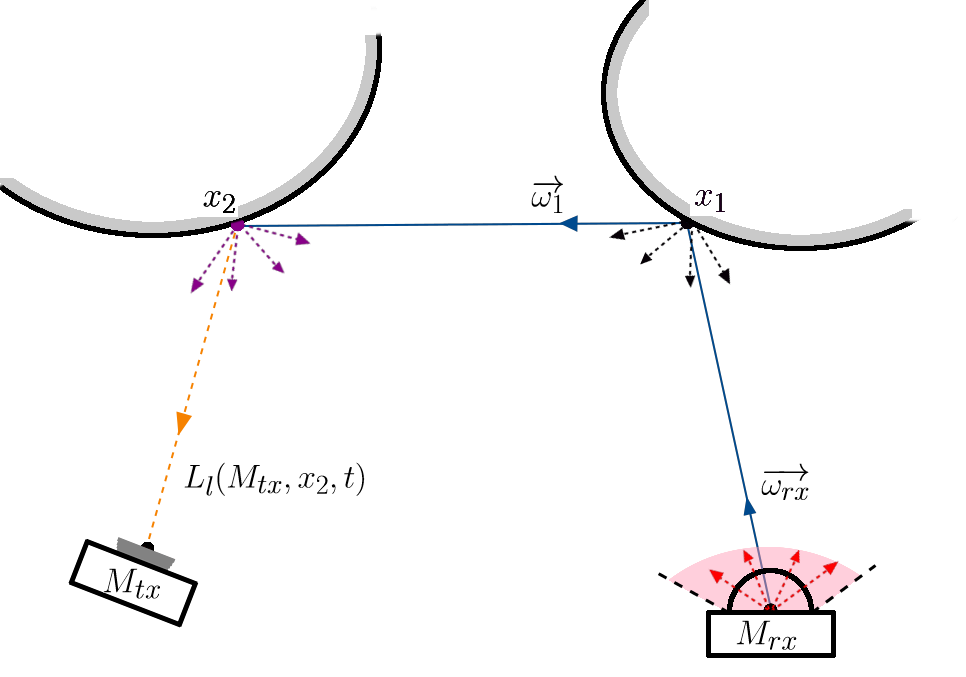
\includegraphics[width=150mm]{LTE_rendu.png}
\caption{Algorithme de rendu pour $k=2$ réflexions}
\end{figure}

Similairement à l'équation en potentiel, on va pouvoir en déduire l'éclairement reçu en un point $x$ après $k$ réflexions.\par
Après $k$ réflexions, on connecte le point de surface $x_k$ au récepteur. Ceci est représenté par la luminance rayonnée depuis l'émetteur $M_{tx}$ et reçue au dernier point de réflexion $x_k$ :
\large \begin{equation}
    L_l(M_{tx}, x_k, t) =
        L_e(M_{tx}, \overrightarrow{M_{tx}x_k}, t)
        V(x_k, M_{tx})
        \frac
            { | \overrightarrow{M_{tx}x_k}\cdot\overrightarrow{n_{tx}} | }
            { \| \overrightarrow{M_{tx}x_k} \| ^3}
.\end{equation} \normalsize \par
On rappelle que $V(x_k, M_{tx})$ est la fonction de visibilité qui vaut 1 si les points $x_k$ et $M_{tx}$ sont visibles l'un l'autre, 0 sinon.\newline\par

Nous voulons connaître l'éclairement reçu au récepteur, par le point de réflexion $x$. L'équation de rendu nous permet de modéliser la luminance réfléchie au point $x_1$ dans la direction $\overrightarrow{x_1 M_{rx}}$. En déroulant cette équation, nous arrivons pour $k$ réflexions à l'équation suivante :
\large \begin{equation}
    E_k(x_1, M_{rx}, t) =
        \int_{\textcolor{red}{\Omega_0}}
            \cdots
            \int_{\textcolor{purple}{\Omega_k}}
                g_k(\textcolor{blue}{\bar{x}}, t)
            \textcolor{red}{d\overrightarrow{\omega_0}}
            \cdots
        \textcolor{purple}{d\overrightarrow{\omega_k}}
,\end{equation} \normalsize
où $\bar{x} = (M_{rx}, x_1, x_2, ... , x_k, M_{tx})$ est un trajet partant du récepteur $M_{rx}$ et passant par $k$ points de réflexions avant d'atteindre la source $M_{tx}$. Et la fonction $g_k$ est:
\large \begin{multline}
    g_k(\bar{x}, t) =
        | \overrightarrow{\omega_0} \cdot \overrightarrow{n_{rx}} |
        rect\left(\frac
            {| \overrightarrow{\omega_0} \cdot \overrightarrow{n_{rx}} |}
            {cos(\textcolor{Rhodamine}{FOV})}
        \right) \\
        \times
        \textcolor{BurntOrange}{L_l(M_{tx}, x_k, t)}
        \prod\limits_{i=1}^k
            f_r(x_i, \overrightarrow{\omega_{i-1}} \longrightarrow \overrightarrow{\omega_{i}})
            | \overrightarrow{\omega_i} \cdot \overrightarrow{n_i} |
,\end{multline} \normalsize
où la fonction $rect$ vérifie que la direction $\overrightarrow{\omega_0}$ au champ de vision du récepteur, \\
le produit des BRDF $f_r(x_i, \overrightarrow{\omega_{i-1}} \longrightarrow \overrightarrow{\omega_{i}})$ à chaque point $x_i$ du trajet est un coefficient multiplicateur du dernier rayonnement en $x_k$.


\section{Equation de rendu optimisée}

Dans cet algorithme trivial on doit doit itérer plusieurs fois sur le même chemin si l'on souhaite avoir les contributions de chaque point de réflexion $x_i$ ($1 \leq i \leq k$) recevant directement de la lumière l'émetteur. On va donc, tout comme pour l'équation en potentiel, relier chaque point de réflexion à l'émetteur. Pour chaque point de réflexion $x_i$, si celui-ci peut recevoir une lumière directe de la source, la contribution de celle-ci est ajoutée avant de tirer une nouvelle direction aléatoire pour aller trouver un autre point de réflexion $x_{i+1}$.\newline\par

L'estimateur de Monte Carlo de cette version améliorée est le suivant :
\large \begin{multline}\label{eq:MC_LTE_rendu}
    E_k(M_{tx}, M_{rx}, t) =
    \frac{1}{N}
    \underbrace{
        \sum\limits_{s=1}^N \frac
            {| \overrightarrow{\omega_{rx}} \cdot \overrightarrow{n_{rx}} |}
            {p_0(M_{rx}, \overrightarrow{\omega_{rx}})}
        }
        _{\textcolor{DarkGray}
         {\substack{\text{On tire une première} \\
                    \text{direction pour $\overrightarrow{\omega_{rx}}$}}}}
    \\ \times
    \sum \limits_{i=1}^k
    \left(
        \underbrace
            {L_l(M_{tx}, x_i, t)}
            _{\textcolor{DarkGray}
             {\substack{\text{Contribution de} \\
                        \text{la source sur le} \\
                        \text{point $x_i$}}}}
        \underbrace
            {\prod\limits_{j=1}^i
                \frac
                    {f_r(x_j, \overrightarrow{\omega_{j-1}} \longrightarrow \overrightarrow{\omega_{j}})
                    | \overrightarrow{\omega_j} \cdot \overrightarrow{n_j} |}
                    {p_j(x_j, \overrightarrow{\omega_{j}})}}
                _{\textcolor{DarkGray}
                 {\substack{\text{Prise en compte de toutes} \\
                            \text{les BRDF des surfaces interceptées} \\
                            \text{par le chemin aux points $x_i$}}}}
    \right)
.\end{multline} \normalsize